\section{Aufbau}
\label{sec:Aufbau}
\begin{figure}[H]
         \centering
         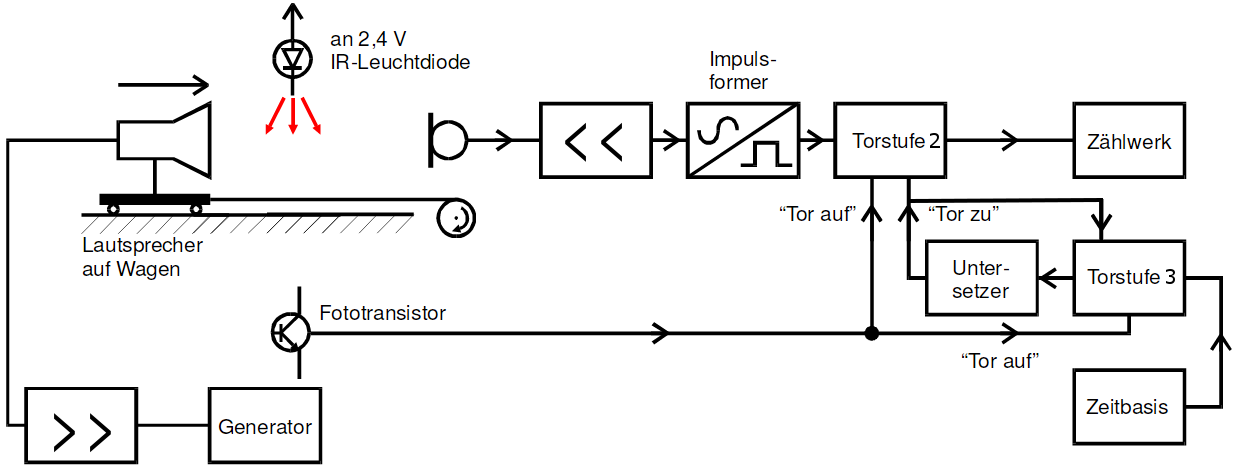
\includegraphics[width=\linewidth-50pt,height=\textheight-50pt,keepaspectratio]{content/Bilder/steve.png}
         \caption{Messapperatur zur Geschwindigkeitsbestimmung der einzelnen Motorgänge, sowie zur Frequenzbestimmung von monofrequenten Schallwellen \cite{V104}.}
         \label{fig:Aufbau}
       \end{figure}

Um die Geschwindigkeitsabhängigkeit einer Schallfrequenz zu ermittteln wird ein Aufbau nach \ref{fig:Aufbau}
 verwendet. Dabei sind der Aufbau zur Geschwindigkeitsmessung und der zur
  Frequenzmessung im Kern derselbe. Dieser besteht aus einem Lautsprecher, welcher
   auf einem an einer Schiene befestigten Wagen moniert ist.
 Dieser ist über eine Seilhalterung mit einem Motor verbunden, mit welchem sich
  der Wagen mit einer konstanten Geschwindigkeit auf der Schiene bewegen lässt.
   Der Wagen lässt sich zehn in Geschwindigkeitsstufen bewegen.
Zusätzlich sind zwei Lichtsensoren, bestehend aus einer Infarot-Lichtquelle und
 einer Photodioden, an der Schiene angebracht.
 Nun zu den Eigenheiten der anfänglichen Zeitmessung. Sowohl Mikrofon als auch
  Lautsprecher sind noch mit einer Torstufe verbunden. Diese ist mit beiden Photodioden verknüft.
    Durchfährt der Wagen
 den ersten Infarotstrahl, wird dieser unterbrochen und die Photodiode sendet ein Signal.
 Mit diesen wird die Torstufe geöffnet. Durchfährt er die zweite wird sie wieder
  geschlossen. Die Zeitdifferenz wird mithilfe eines Zählwerkes ermittelt.
    Eine mögliche Schaltung zum ööfnen und schließen
  der Torstufe ist in Abb. AAAAAAAA dargestellt.
  Zur Frequenzmessung wird das Mikrofon über einen Impulsformer mit einem Zählwerk
   verbunden, welches die empfangenen Impulse, also die Anzahl der am Mikrofon empfangenen Schwingungen zählt.
   Um nun eine Frequenz zu ermitteln wird eine feste Messzeit eingestellt. Hierzu öffnet
   eine Lichtschranke beim durchfahren des Wagens zwei Torstufen. Die erste
    startet das oben beschriebene Zählwerk, die zweite startet einen Untersetzer.
     Dieser zählt anschließend mit einem Zeitbasisgenerator von einer fest gesetzten Zahl herab.
      Fällt diese auf Null wird die erste Torstufe wieder geschlossen. Ein Schaltplan
       beider Torstufen ist in Abb. AAAFSFDSD dargestellt.
       \begin{figure}[H]
                \centering
                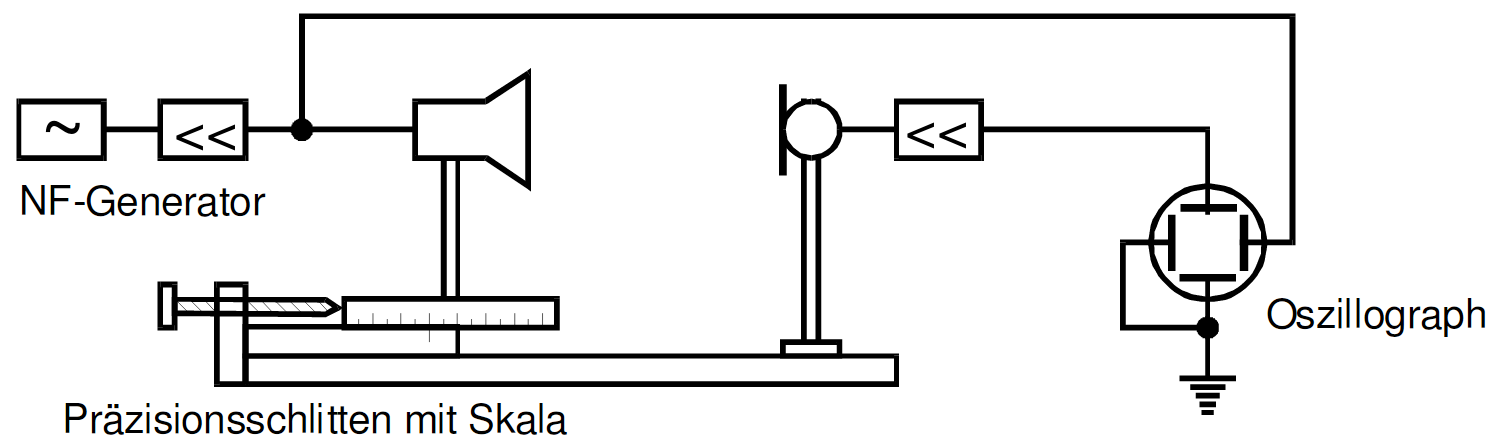
\includegraphics[width=\linewidth-50pt,height=\textheight-50pt,keepaspectratio]{content/Bilder/Lambda.png}
                \caption{Messapperatur zur Bestimmung der Wellenlänge einer Schallwelle \cite{V104}.}
                \label{fig:lamb}
              \end{figure}

       Zuletzt wird ein zweiter Aufbau wie in \ref{fig:lamb} zur Messung der Wellenlänge verwendet.
       Dieser besteht aus dem Lautsprecher, welcher diesmal in einer Mikrometerschraube fixiert
        ist und dessen Signale zusätzlich auf einm Ossziloskop dargestellt werden.
        Am anderen Ende der Schraube steht ein Mikrofon, welches die Schallwellen an einen zweiten Eingang
         des Ossziloskops sendet. Auf dem Ossziloskop werden beide Signale überlagert.
